\documentclass[a4paper,12pt]{article}
\usepackage[utf8]{inputenc}
\usepackage{amsmath}
\usepackage{amsthm}
\usepackage[utf8]{inputenc}% acentos sin codigo
\usepackage[activeacute,spanish]{babel} %acentos sin código
\usepackage{geometry}
\geometry{top=1.8cm, bottom=2cm, left=2.5cm, right=2.5cm}
\usepackage{graphicx}
\usepackage{subfigure}
\usepackage{fancyhdr}
\usepackage{cite}
\usepackage{dsfont}
\usepackage{mathrsfs}
\usepackage{lscape}
\usepackage{enumerate}
\usepackage{ulem}
\usepackage[spanish]{babel}
\usepackage{color}
\usepackage{cancel}
\usepackage{multirow,array}
\usepackage{float}
\usepackage{lscape}
\usepackage{rotating}
\date{\today }
\title{}
\author{Victor Valladolid Onecha}
\begin{document}
\renewcommand{\tablename}{Tabla}


\begin{figure}
\centering
\subfigure[Agua $100\%$]{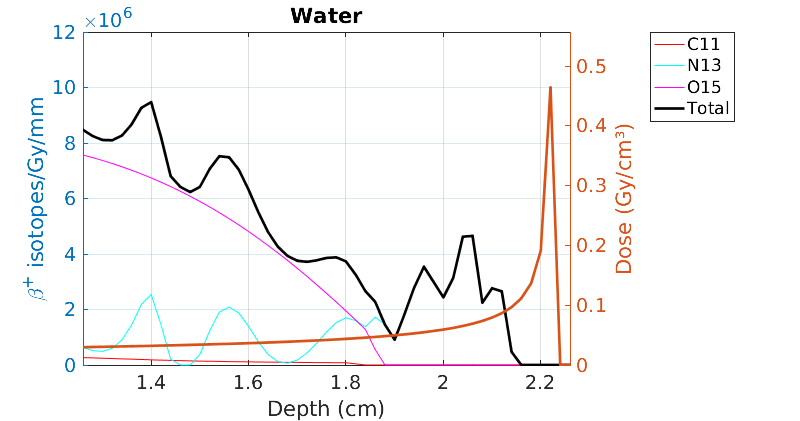
\includegraphics[width=0.7\textwidth]{water.png}}
\subfigure[Agua $90\%$+ Iodo $10\%$]{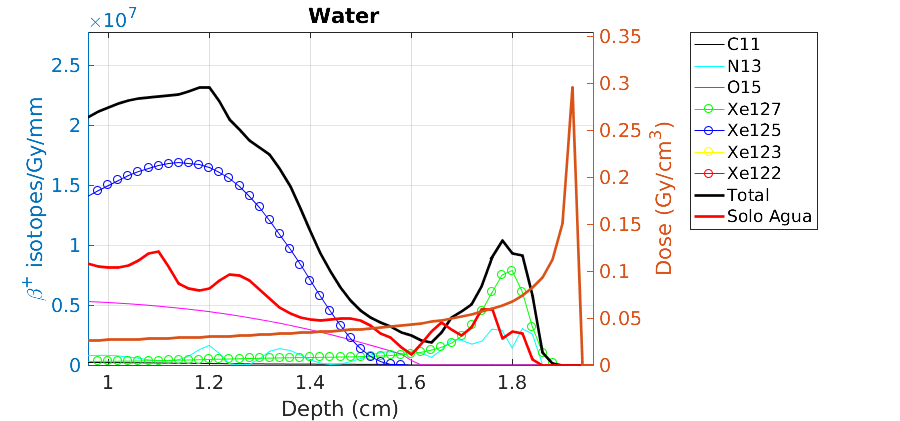
\includegraphics[width=0.7\textwidth]{water_i_10.png}}
\subfigure[Agua $85\%$+ Iodo $15\%$]{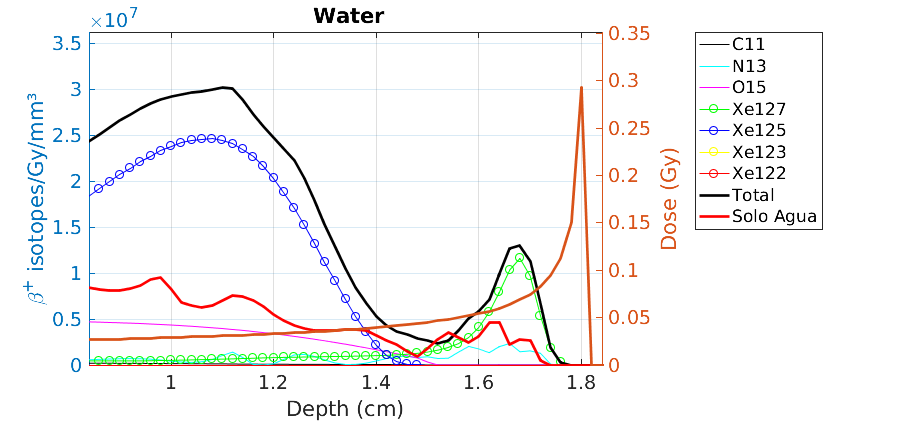
\includegraphics[width=0.7\textwidth]{water_i_15.png}}
\end{figure}



\begin{figure}
\centering
\subfigure[Piel $100\%$]{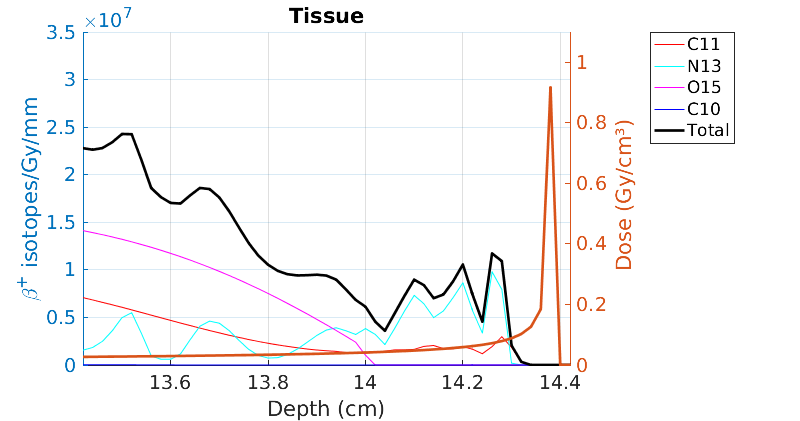
\includegraphics[width=0.7\textwidth]{tissue.png}}
\subfigure[Piel $90\%$+ Iodo $10\%$]{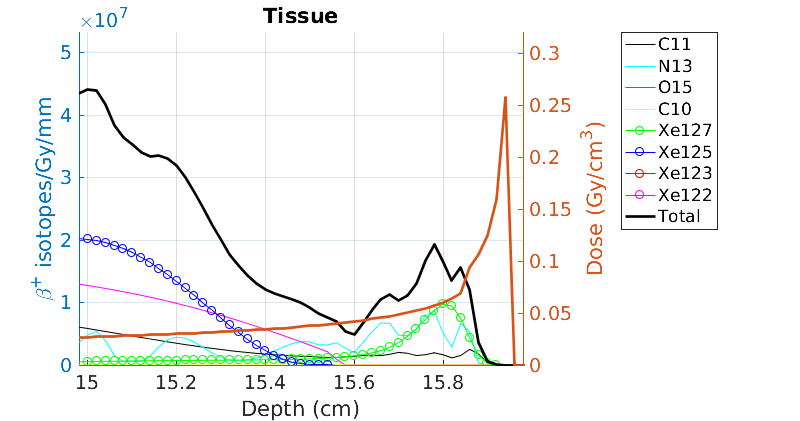
\includegraphics[width=0.7\textwidth]{tissue_i_10.png}}
\subfigure[Piel $85\%$+ Iodo $15\%$]{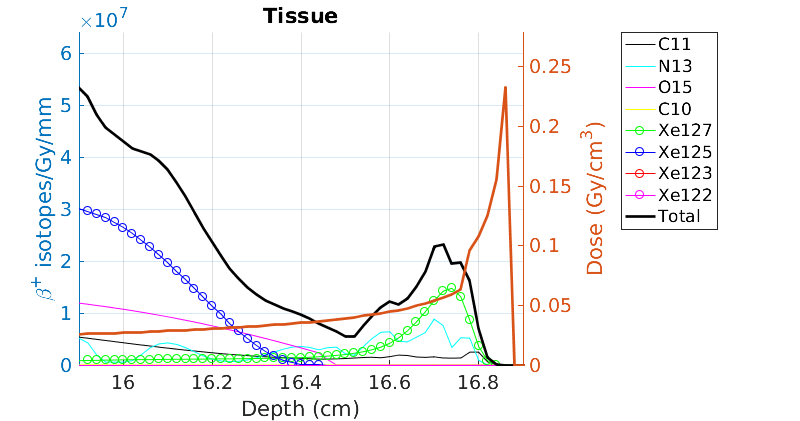
\includegraphics[width=0.7\textwidth]{tissue_i_15.png}}
\end{figure}




\begin{figure}
\centering
\subfigure[Grasa $100\%$]{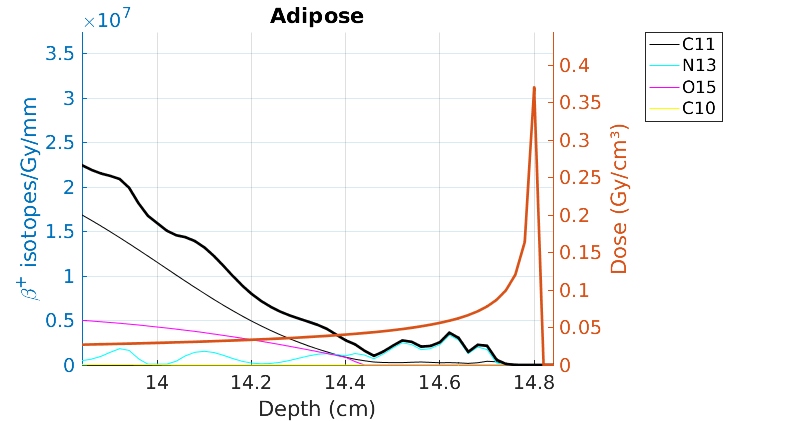
\includegraphics[width=0.7\textwidth]{adipose.png}}
\subfigure[Grasa $90\%$+ Iodo $10\%$]{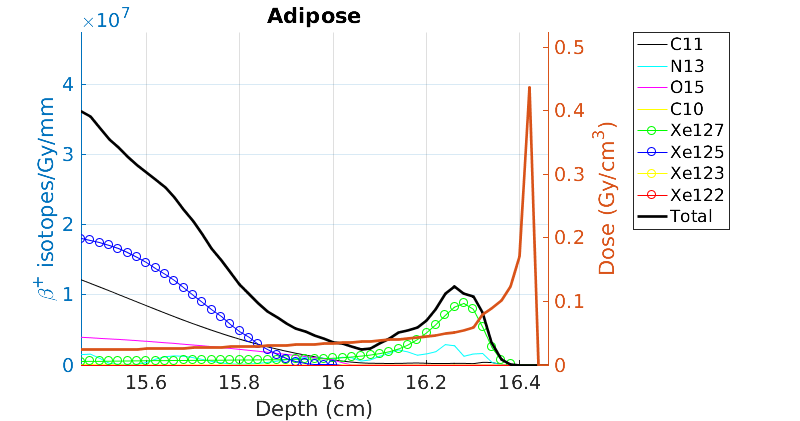
\includegraphics[width=0.7\textwidth]{adipose_i_10.png}}
\subfigure[Grasa $85\%$+ Iodo $15\%$]{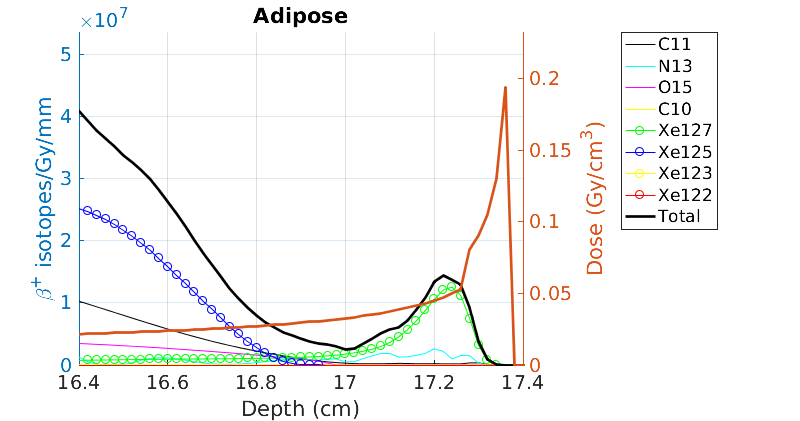
\includegraphics[width=0.7\textwidth]{adipose_i_15.png}}
\end{figure}





\begin{figure}
\centering
\subfigure[Hueso $100\%$]{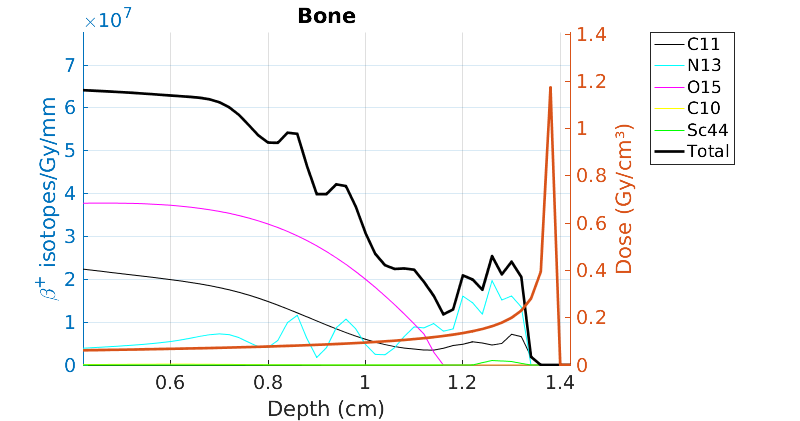
\includegraphics[width=0.7\textwidth]{bone.png}}
\subfigure[Hueso $90\%$+ Iodo $10\%$]{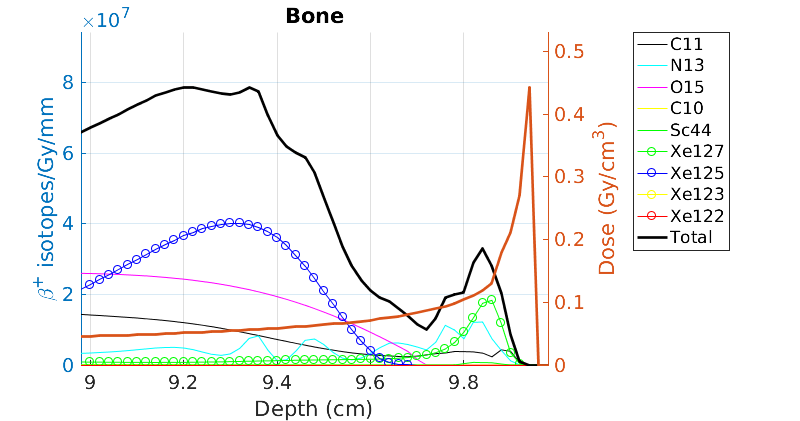
\includegraphics[width=0.7\textwidth]{bone_i_10.png}}
\subfigure[Hueso $85\%$+ Iodo $15\%$]{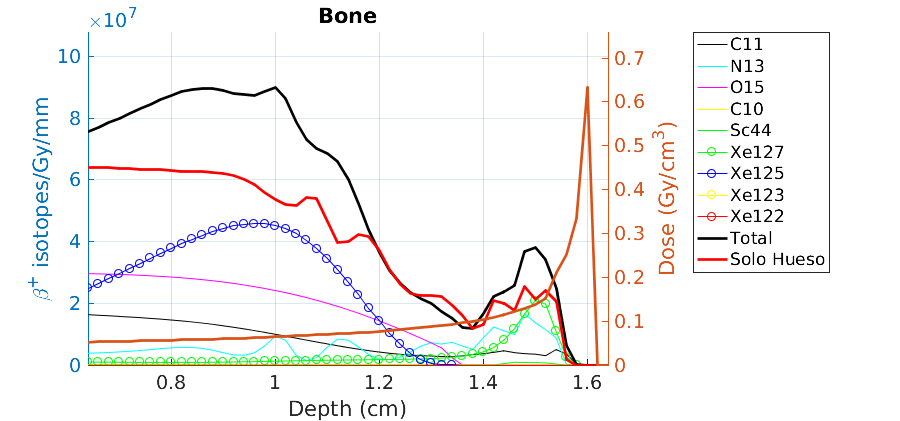
\includegraphics[width=0.7\textwidth]{bone_i_15.png}}
\end{figure}




















\end{document}